\chapter{Models@Runtime for the IoT}
\label{ch:MARContiki}
%As presented in chapter \ref{ch:IoT}, Internet of Things systems are typically formed by a myriad of many small interconnected devices.
%This underlying hardware infrastructure raises new challenges in the way we administrate the software layer of these systems.
%Indeed, the limited computing power and battery life of each node combined with the very distributed nature of these systems, greatly adds complexity to distributed software layer management.
Taking into account the distributed nature of the IoT environment, we can observe that deployment of new functions and updates for bug fixing is a very challenging task.
%The capacity of dynamically deploying and reconfiguring the software layer on the IoT is a crucial feature.
Thus, designing a tool able to provide such capacities in this constrained context raises several scientific challenges.
All the following challenges are related to the limited resources of these nodes and the particular topology of the network that interconnect them.
We address the problem of enabling the deployment of a distributed software layer and its dynamic reconfiguration over a network of nodes featuring very limited resources: memory, processing power, bandwidth communication and energy autonomy.
%Therefore, a simple adaptation of an existing implementation for deployment and reconfiguration in distributed systems would not fit on a typical IoT device.
%Indeed, the very scarce resources limits the use of complex approaches \textit{"as is"}, as it was already described in section \ref{sec:dynamicDeploymentDAS}

% limitation of SOTA
Looking at our state of the art, various techniques have been proposed to enable software updates, which were presented in table \ref{tab:deployMethods}.
As for the full kernel replacement mechanism, which can be managed by an automatic tool\cite{hui2004dynamic}, the excessive amount of power needed by this approach does not seem appropriated for a highly dynamic infrastructure such as the IoT.
The approaches making use of virtual machines were already analyzed and it was found that they are not suitable for long-living applications\cite{oliver2014reprogramming}.
Even if some component models \cite{mottola2008figaro}, \cite{taherkordi2013optimizing} were proposed to provide an abstraction layer for the life-cycle maintenance, it results in a very complex programming model and routing protocols to distribute components, in addition to a finely tuned memory manager for specific platforms and hardware architectures, which reduces scalability.
Thus, the lack of a deployment manager leveraging kernel modularization using relocation mechanisms, which seems the best way to provide new features and updates, motivates our research to find an automatic and scalable approach to provide such a manager.

%Indeed, the previously studied models@runtime approach, and more specifically, the Kevoree approach, provides a way to manage the application layer for distributed systems.
%As stated in section \ref{sec:distDeployment}, the high resemblance between distributed systems and the IoT, makes the use of such approach a viable solution.
%However, the huge differences in computing capacity and energy autonomy between the nodes involved in both scenarios make the implementation of this approach very challenging.
%Thus, a direct mapping of Kevoree (the meta-model and its model manipulation tools) cannot be foreseen.

In this chapter, we describe the main challenges while implementing a new middleware dedicated to IoT devices, in order to enable the management of software deployment and the dynamic reconfiguration of IoT systems.
Indeed, our middleware is inspired from the Component Based Systems and the model@runtime paradigm which have been already described in the previous chapter.
%Moreover, our proposition is based on an existing implementation of the paradigm of models@runtime which has been adapted to fit IoT devices constraints.

%Moreover, the implementation of this middleware follows the directions of the existing Kevoree meta-model depicted in \todo{annex or figure?}, which has been adapted to fit IoT devices constraints. 
As a matter of fact, our evaluation of these constraints was conducted on several hardware platforms typical of the IoT, in order to establish a reference for the minimum requirements to run such a middleware.
%Once an initial research on these IoT platforms was conducted, the proposition of a new one was necessary, since the minimal requirements were not met by the commercially available platforms at that time.
%Such platform was an essential part to evaluate our first implementation, and was used to establish the minimum requirements of an execution environment.
%Finally, we have conducted the evaluation of our approach on an Internet of Things testbed\cite{Fleury15iotlab} recently available for experimentation.
%Our results demonstrates the feasibility of providing a model@runtime middleware for these systems, which can be executed in platforms meeting the requirements already established.
%This chapter is concluded by the obtained results on the FIT IoT-Lab testbed, which show the limits of our first approach.

\section{Requirements from IoT  for a Models@Runtime implementation}
\label{sec:MARMech4IoT}
Looking into the Models@Runtime approach, we can observe that some of the provided functionalities can be leveraged in order to ease software distribution and deployment in a distributed system.
We can take these basic functionalities to perform the following tasks:

\begin{enumerate}
	\item Detect and decide which part of the model should evolve.
	\item Find the right software components to adapt the system into the new requirements.
	\item Deploy this new components into the right nodes.
\end{enumerate}

In order to accomplish these tasks, we need to implement the mechanisms provided by this approach, specifically for deployment and reconfiguration.
Indeed, we can divide them into software and hardware capabilities.
Thus, the following software requirements would allow a functional models@runtime implementation:

\begin{enumerate}
	\item A running software representation, divided in components. Preferably in a form of separated processes (threads, protothreads) list.
	\item A dynamic loading mechanism to update or add new software matching the new requirements (adaptation, reconfiguration).
	\item A way to disseminate the serialized model, software components and to exchange messages (networking).
\end{enumerate}

As we have already discuss in the state of the art on section \ref{sec:DSOverview}, these are the typical characteristics of a distributed system. 
Indeed, the IoT fulfill all these requirements, which are often implemented in the form of IoT operating systems, already presented on section \ref{sec:IoTOS}.
Moreover, they also provide support for several IoT platforms, allowing and facilitating support for new ones.
Thus, for our needs, we can establish the following requirements in terms of hardware:

\begin{enumerate}
	\item A Micro-Controller Unit (MCU) big enough in terms of memory size (ROM and RAM) to support the software needs. It should also provide different low power consumption modes.
	\item A networking interface (radio) providing wireless communication means with low power (sleep) modes.
	\item External (flash) storage for software updates and new modules.
\end{enumerate} 

Given the software and hardware requirements, we need to address them by either using existing software and run it into an existing hardware platform, or by developing new ones.
We will first analyze the minimum software requirements for a specific M@R implementation, already presented as the Kevoree Framework, followed by the minimum hardware requirements to run such implementation.

\section{Kevoree as a flexible models@runtime approach}
\label{sec:MAR_overview}
The Kevoree framework, which was already introduced in subsection \ref{subec:kevoree}, is composed by a meta-model which describes the main parts of a distributed system, coupled with a minimalistic component model.
A typical Java implementation of this meta-model consists in code generated by common modeling tools, such as the Eclipse Modeling Framework (EMF)\cite{steinberg2008emf}, resulting in a vast quantity of code representing all the classes and its relationships.
Even if big efforts to reduce the generated code and dependency resolution complexity present in EMF were conducted by Fouquet \textit{et al.} in \cite{fouquet2012eclipse}, the need of a JVM and a big amount of memory are still the main inconvenient for their use on the IoT.
Moreover, the principle of a model@runtime lies in the general knowledge of the entire system (the reflected model of the running system), which is present in every participant.
Indeed, the reflected model should be available in memory for its rapid manipulation, thus we can imagine the big quantity of memory needed to represent large models featuring a vast quantity of nodes.
In addition, each node can have instances of one or more components and its parameters, which increase even more the size of the model in memory.
It is then very complex and challenging to provide such a framework on the context of IoT.

\begin{figure}[]
	\centering
	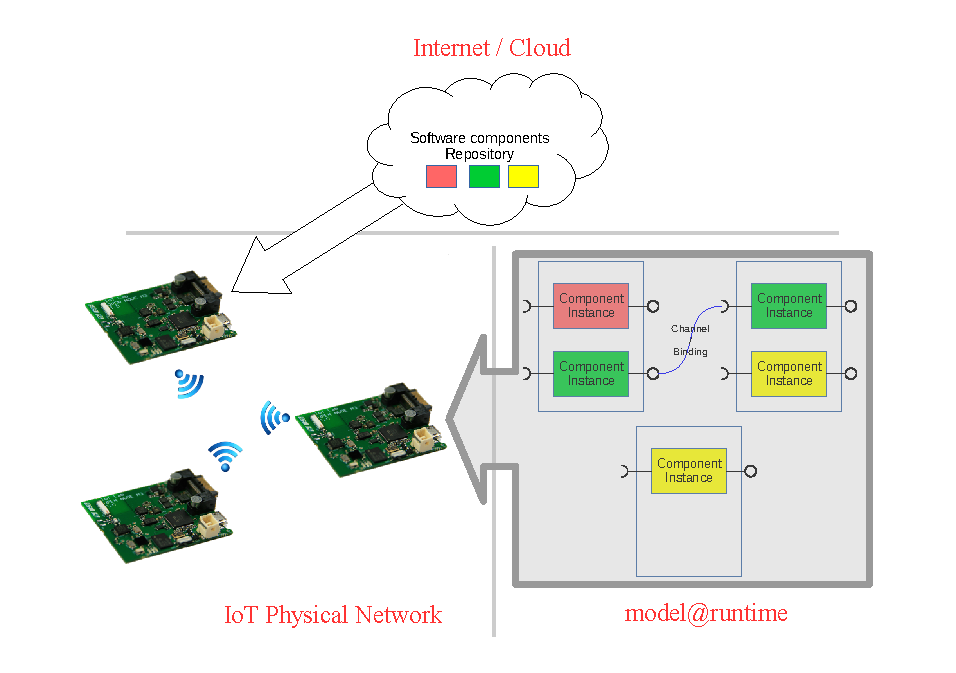
\includegraphics[width=1\columnwidth]{chapters/modelsAtRuntimeContiki.images/MAR_IOT.pdf}
	\caption{A M@R representation for IoT devices}
	\label{fig:MAR_IOT}
\end{figure}

However, some of the Kevoree activities are interesting for their use on a distributed environment such as the IoT.
Indeed, Kevoree is able to perform reconfiguration and deployment tasks, which are the main functionalities we are searching for.
To be precise, the implementation provides:

\begin{itemize}
	\item \textbf{The meta-model to represent the whole distributed system.} The representation proposed by Kevoree through the meta-model is very close to our IoT environment, since it focuses on independent nodes and provides abstractions for the communication means, which is the main activity of an IoT node.
	\item \textbf{Principles for model manipulation.} Several tools are needed while changes on the system are reflected on the model. It is then needed to change parameters, add or remove components, check for changes between old and new models and so on. Thus, tools like model serializer/deserializer, model comparing, and model visitors, are essential for a functional Kevoree implementation.
	\item \textbf{Kevoree editor} A web editor is available for model checking/editing. This is very useful while triggering adaptations by hand.
\end{itemize}

Our goal is then to provide a middleware that will be present on each node of the IoT system, and will take care of the various tasks imposed by the model@runtime paradigm.
In figure \ref{fig:MAR_IOT} we can see a representation in which three IoT nodes are part of a small network.
This example shows a M@R which is present on the three nodes, each node has the knowledge about three available components on the repository, the instances present in the other two nodes and a binding through a channel between two components of different nodes.
Any change of this configuration should be reflected on the model, followed by the dissemination of these changes to the other nodes, and vice-versa, any change on the model will affect the actual node.
Figure \ref{fig:MAR_reconfig} describes the actions taken when a reconfiguration or adaptation is triggered.

\begin{figure}[]
	\centering
	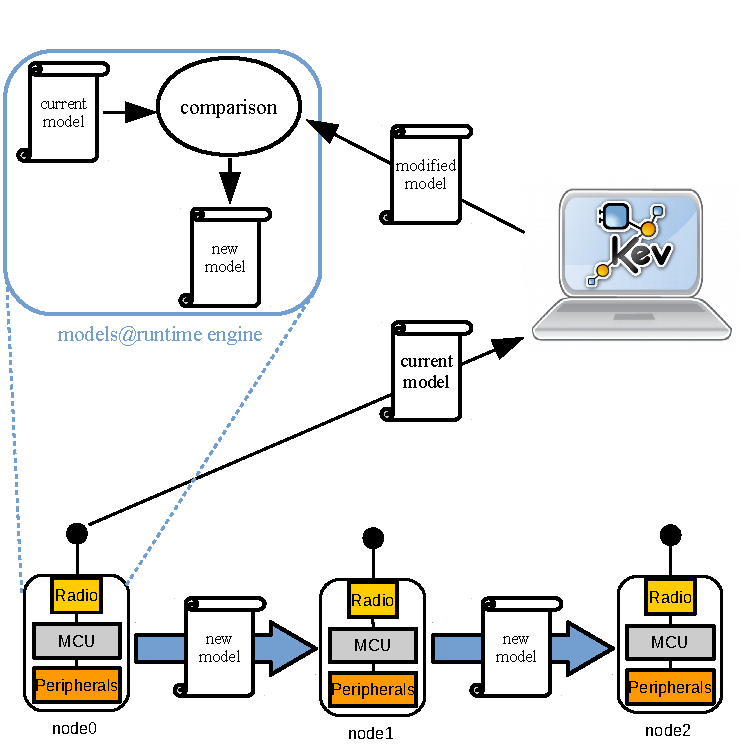
\includegraphics[width=1\columnwidth]{chapters/modelsAtRuntimeContiki.images/reconfigMAR.pdf}
	\caption{Reconfiguration through a M@R}
	\label{fig:MAR_reconfig}
\end{figure}

%Following the directions presented above, an implementation of this approach on IoT nodes has been conducted, which should be able to have a similar model representation in memory and to enact the adaptation and reconfiguration process on each node.
As we stated before, the exact implementation of the Kevoree M@R approach using the current tools is not feasible, due to the IoT node's constraints.
Thus, we need to leverage only the most important mechanisms provided by this approach, and adapt the selected features to address the node's hardware constraints.
It is also important to offer a similar behavior and interoperability with the other Kevoree implementations.

\section{Kevoree for the IoT}
\label{sec:kevAndIoT}
The Kevoree framework is composed by several parts which provide a complete models@runtime implementation.
The base of this framework is the Kevoree meta-model, which was designed to follow a distributed architecture and a minimalistic component model.
Thus, a first challenge lies in the implementation of such meta-model meeting the programming language and memory constraints.

\subsection{Minimal Kevoree properties needed on the IoT}
\label{subsec:minKevProp}
As already discussed in section \ref{sec:MAR_overview}, the Kevoree meta-model can be easily transformed into Java code using a modeling framework.
However, in our case this approach cannot be used.
This is due to two reasons: first, we cannot use high-level languages such as Java and second, we are limited to the C language which can be compiled for the IoT node's architecture already presented in \ref{subsec:smartObjects}.
Moreover, meta-models follow very often an object-oriented approach, which is not defined for procedural languages such as C.
Thus, a direct transformation taking into account this constraints is not worth considering.
However, a similar approach for code generation and modeling tools can be proposed to meet the requirements of a model@runtime approach.
Indeed, the Kevoree Modeling Framework\cite{fouquet2012eclipse} can be adapted to support the generation of C code, in order to provide a fully Kevoree-like middleware for IoT devices.
Even so, the efforts to adapt such a framework raise more and different challenges that are out of the scope for this thesis.
Since our goal is to, first of all, investigate the limits of an IoT node in terms of memory, a manual implementation (transformation) of the meta-model and its modeling tools was conducted, adapting the concepts to the limited resources of the node.
Indeed, this allows a rapid prototype which can be finely tuned to meet the memory constraints present in IoT devices, in contrast to a more generic code generation approach.

On the typical implementation of Kevoree, a \textit{core} application is embedded in every node. 
This application provides to each system element (node, component, communication channel, groups) an access to the current model, allowing to submit new configurations through new models.
If this \textit{Kevoree Core} receives a new model, it is in charge of the validation, then the adaptation planning and finally the execution of this adaptation.
In figure \ref{fig:MAR_reconfig} we can observe a reconfiguration triggered by the Kevoree editor, which is able to modify the model retrieved from a node.  The set of adaptation stages mentioned above are then carried through a transactional manner.

The model validation is delegated to any system element registered as a \textit{listener}.
Each component, communication channel or node can make use of an interface and be registered on the \textit{core} in charge of the model management.
Once registered, the instance is notified with regard to the different reconfiguration stages.
For this, a \textit{listener} interface can define the following notifications:
\begin{itemize}
	\item \emph{preUpdate} allows to the \emph{listener}s to be notified that an update has been proposed.
	Each \emph{listener} can then validate the proposed configuration.
	\item \emph{preAllUpdate} allows to the \emph{listeners} to be notified that the proposed update has been validated by the set of \emph{listener}.
	\item \emph{postUpdate} allows to the \emph{listeners} to be notified that the update has been applied.
	Each \emph{listener} can then validate that the update does not cause a problem.
	\item \emph{postAllUpdate} allows to the \emph{listeners} to be notified that the update which has been applied was also validated by the set of \emph{listener}s.
	\item \emph{preRollback} allows to the \emph{listeners} to be notified that the update has failed and a rollback to the previous configuration will be carried out.
	\item \emph{postRollback} allows to the \emph{listeners} to be notified that the rollback has been successful.
\end{itemize}
Figure \ref{fig:MAR_modelListener} represents in a state-transition diagram the integrations of \textit{listeners} with the process of \textit{model@runtime}.

\begin{figure}[]
	\centering
	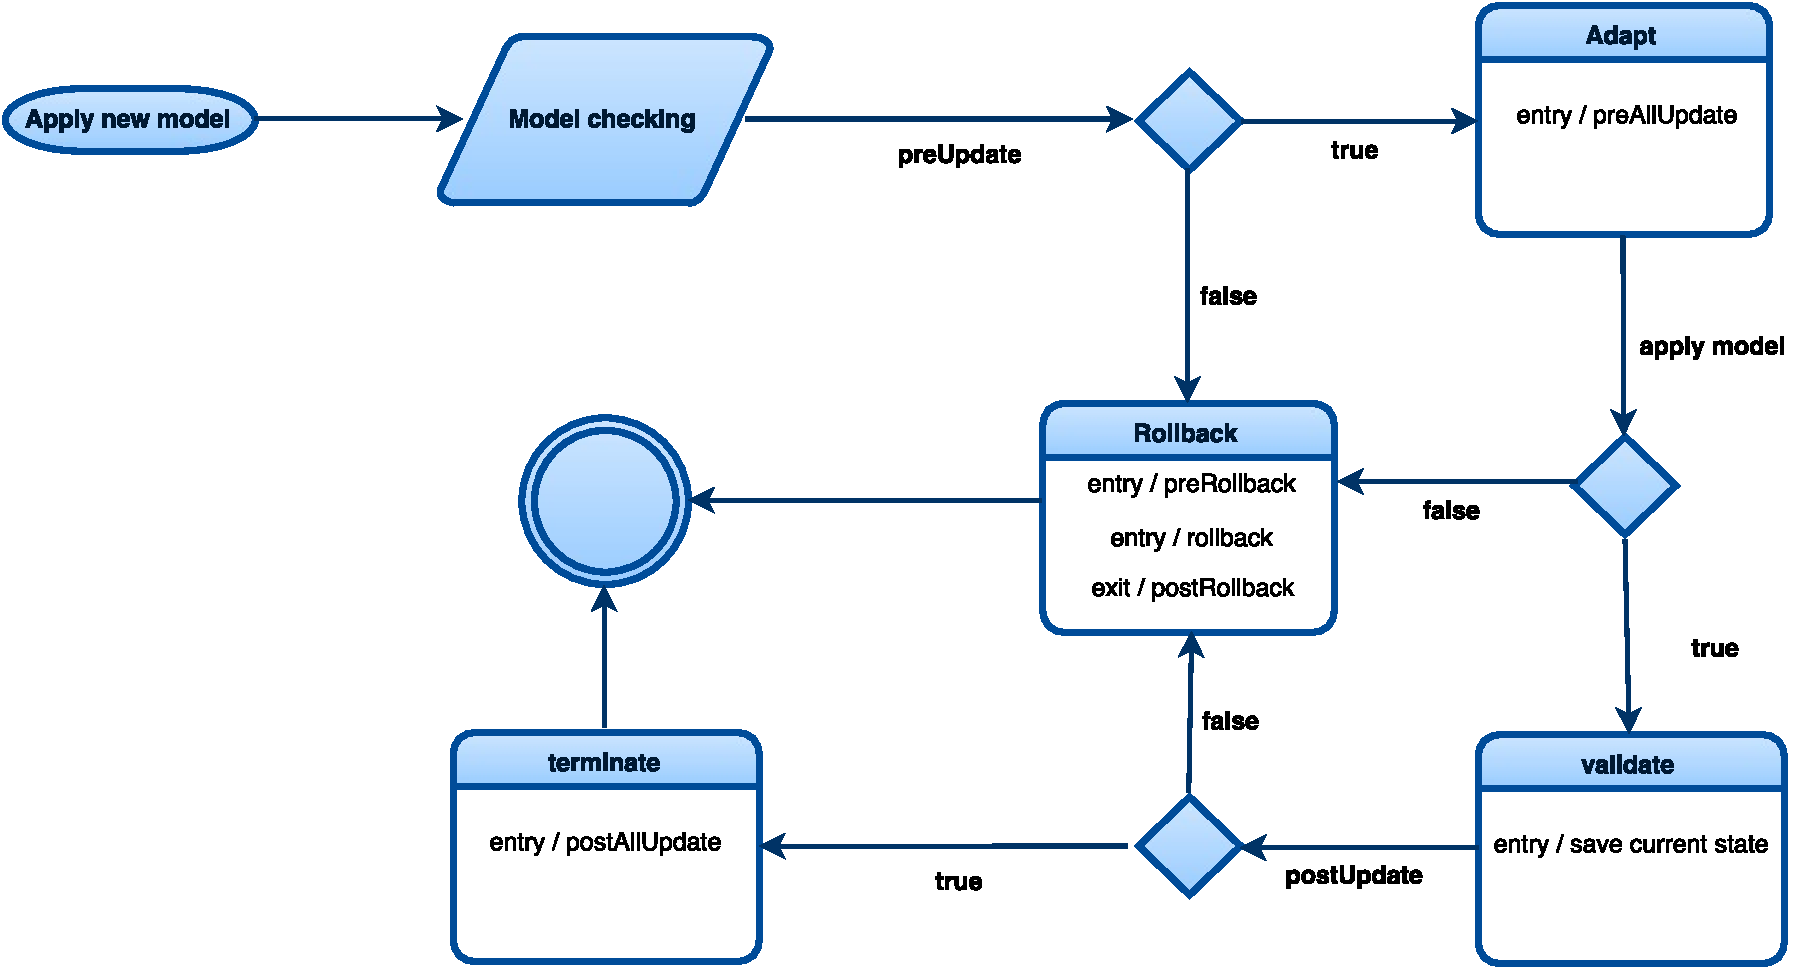
\includegraphics[width=1\columnwidth]{chapters/modelsAtRuntimeContiki.images/ModelListenerStateChart.pdf}
	\caption{State-transition diagram showing the integration of ModelListeners in the M@R process}
	\label{fig:MAR_modelListener}
\end{figure}

In contrast, our implementation for IoT devices cannot follow the same approach.
Indeed, the model checking and rollback mechanisms require to save the entire model in memory for checking and, if something goes wrong, to bring back the previous model.
This is very memory consuming for our application.
Therefore, only a simple model checking followed by the adaptations execution has been implemented.
%Moreover, the implementation of this mechanism for all the system elements (component, communication channel, group) was not necessary for our first prototype.
Thus, only a \textit{ModelListener} is present on our core, avoiding all the notification process, saving processing time thus energy.
Indeed, in our proposition the node is in charge of the adaptation mechanisms, since for our concerns (an IoT system) nodes are the main component and it can only execute an instance of itself.
This vision contrast with a typical Kevoree implementation, where various \textit{Kevoree Core} can run in a single machine, resulting in several nodes reflected in the model.

%In conclusion, our proposition for a Kevoree implementation on IoT devices is conceivable, since we bring the most important features with a very low memory footprint, having only a few limitations.


\begin{figure}[]
	\centering
	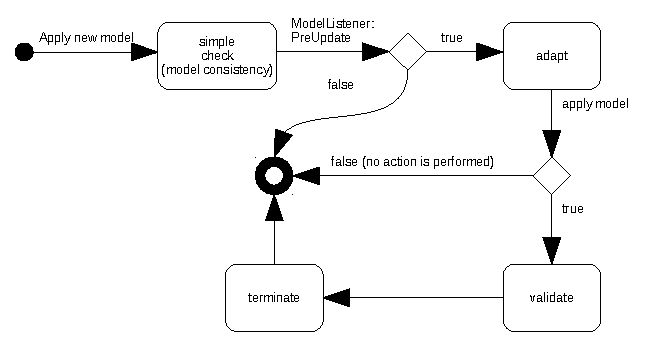
\includegraphics[width=0.85\columnwidth]{chapters/modelsAtRuntimeContiki.images/modelListenerIoT.pdf}
	\caption{State-transition diagram showing the integration of ModelListeners in the M@R process for IoT devices}
	\label{fig:MAR_modelListenerIoT}
\end{figure}

Figure \ref{fig:MAR_modelListenerIoT} depict the state-transition diagram according to our M@R process for IoT devices.

\subsection{Energy, processing and communication constraints}
\label{subsec:ImplConstraints}
Another concern while adapting the selected features of the Kevoree M@R implementation is the amount of energy needed to run it.
Indeed, an IoT device running on batteries should be able to embed this middleware without a high overhead in terms of energy consumption.
Since the most processor consuming task is the model checking and adaptations execution, a smaller overhead is induced, compared to the traditional approach, thanks to the simplification of such process.
However, it was discussed that the most energy consuming task for an IoT device is the radio communication.
The traditional Kevoree implementation was done having in mind no restrictions for network usage and bandwidth, thus algorithms such as Gossip\cite{fouquet2012dissemination} were used for model dissemination.
The implementation of such a protocol in an IoT device could be very memory consuming, in addition to a high energy consumption while using the network.

Given the energy and memory constraints, a dissemination protocol adapted for IoT devices is then needed.
It results interesting that the already described Deluge protocol\cite{hui2004dynamic} seems to be a good option, since it was developed having in mind the constraints of an IoT device.
As the information to be shared is not as big as an entire firmware, but rather a small serialized file including the model, the needed energy to disseminate a model can be low enough.
Moreover, a compression method using an association table including the most often used keywords has been proposed, reducing the model size by more than a half.
By these means, a small file including the model is shared between all the concerned IoT nodes in the network.

\begin{figure}[]
	\centering
	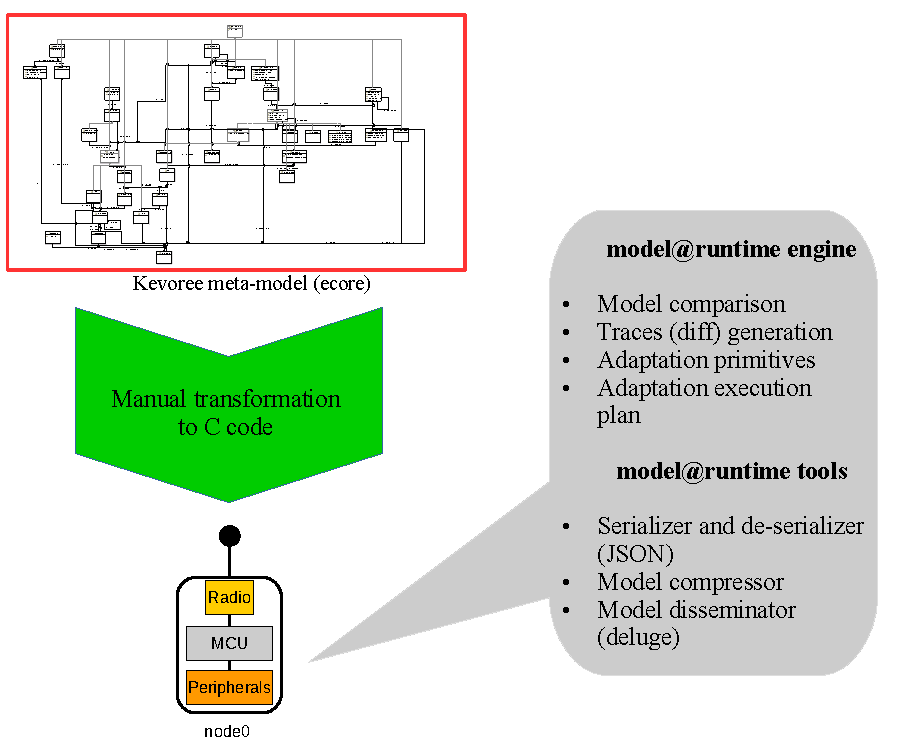
\includegraphics[width=0.85\columnwidth]{chapters/modelsAtRuntimeContiki.images/Challenges.pdf}
	\caption{The two different needs for a complete IoT models@runtime engine}
	\label{fig:MAR_Challenges}
\end{figure}

\subsection{Implementation review and challenges}
\label{subsec:implReview}
After describing the main implementation issues and challenges, we can highlight these in figure \ref{fig:MAR_Challenges}.
Indeed, a models@runtime implementation it is not straightforward, and needs special attention to meet the constraints already discussed previously.
In summary, as depicted on figure \ref{fig:MAR_Challenges}, we have two aspects which result in a complete M@R implementation: the kevoree meta-model, which describes the model representation of the current system, as well as the component model, and the M@R engine which manipulates this model.
This engine was developed having in mind all the constraints present in an IoT device, and at the same time provides the main functionalities to receive, compare and generate a list of found differences (traces) between the current model and a (modified) new one.
Moreover, in order to receive and send models through the network, a serializer and de-serializer is needed, using a JSON format.
In addition, a model compressor and an adaptation of Deluge as a dissemination tool, already discussed in Subsection \ref{subsec:ImplConstraints} are also provided.
In conclusion, our middleware would be able to provide a list of needed adaptations, based on predefined adaptation primitives, such as add/remove components, change dictionary entries (parameters) and stop or start component instances.
Finally, an ordered plan to execute such adaptations is given to the actual system, which will perform the actions.
Therefore, we can now separate our approach into two different challenges.
The first one, which is the meta-model and modeling engine implementations.
The second one, the system facilities development to enact the adaptations provided by the M@R engine.

As stated in section \ref{sec:MARMech4IoT}, in order to provide a complete middleware based on the previous challenges, it is necessary to fulfill the requirements for its implementation in terms of hardware.
A first step is to deploy and test the meta-model implementation and the modeling tools in real IoT motes, in order to measure the memory, energy and latency overheads.

Since this middleware can be very complex, it is necessary to establish the minimal hardware requirements to run it, taking into account the different IoT devices available, already described on Table \ref{tab:DeviceClass}.
The next section will discuss the minimal requirements for this middleware, by analyzing a first implementation and its memory size.
Afterwards, a study on the IoT devices resources is performed, in order to find the IoT devices able to run it, showing the scalability and limitations.

%context
%Based on this principle, IoT dedicated devices have emerged, forming the IoT infrastructure already described in section \ref{sec:IoTInfra}.
%All this new IoT devices form a constellation of many small interconnected objects integrated into houses, building, cities, factory chain, etc.
%Based on this principle, Cyber Physical Systems (CPS) have emerged.CPS are pervasive and long living systems formed by a constellation of many small interconnected devices integrated into houses, building, cities, factory chain, etc. 
%motivation
%In our building automation scenario presented in section \ref{sec:BAScenario}, the described IoT subsystem typically rely on sensor nodes that detect and record data such as presence, temperature, ambient lighting and energy consumption. 
%Thus, the IoT uses sensors to continuously analyse the situation in order to adapt our living environment to match user needs and preferences.
%User wishes may involve different objectives such as comfort, air quality, and energy savings. 
%To go beyond energy management and comfort, building automation systems have to deal with new types of services, depending on the use of the building: fire safety and security management for hotel, indoor air quality control in schools and office buildings, etc. 
%The opportunities of services offered by the IoT and the user preferences are countless and will change over the lifetime of these systems.
%The set of small interconnected devices integrated into buildings can be seen as a computing infrastructure that can host these new services. 
%Consequently the software deployed on these nodes needs to be dynamically reconfigured and re-deployed to meet the evolution of services and user preferences. 


% old sentences
%Consequently comfort and quality are factors of productivity and do not prevent energy savings being achieved.
%To go beyond energy management, building automation systems have to deal with new types of services, depending on the use of the building: fire safety and security management for hotel, indoor air quality control in schools and office buildings etc. 

%problem


%our approach

%plan
%This paper is structured as follows. Section 2 presents the Kevoree component model. Section 3 details the challenges of mapping the model@runtime paradigm to microcontrollers, and explains how we implemented Kevoree on these very limited nodes. Our proposal is evaluated in section 4. Section 5 presents related work and Section 6 gives our conclusion and highlights some perspectives to be addressed in future work.

\section{An empirical study on constrained IoT devices}
The model@runtime paradigm has been mainly investigated in the context of distributed systems. 
These research efforts have been focused on the provision of a comprehensive set of tools to easily deploy, dynamically reconfigure, and disseminate software on a set of distributed computing units.
The current model@runtime tools have been implemented regardless of the specific characteristics and constraints of IoT devices.
In particular, the network topology and the resource constraints of the nodes forming the distributed system have not been taken into consideration.
As a result, state of the art model@runtime tools are not suitable to be used in the context of IoT Systems.
%First, most approaches are relying on the Java language, which does not meet the resource constraints of the computing nodes. 
%Secondly, the size of the model and its distribution among the system are not taking into consideration the limited memory capacity of each node, and their energy constraints.

In \cite{fouquet2012dynamic} $\mu$-Kevoree, the closest effort to port the model@runtime paradigm on the constraints of a Cyber Physical System (CPS) was presented, in which the underlying device is comparable to an IoT device.
Despite the particular attention given to the specific constraints of a Cyber Physical System, this work heavily relies on over the air firmware flashing to support the deployment and reconfiguration of software. 
We consider that relying on firmware flashing to support software deployment constitutes a flaw in the approach because of its energy cost (the complete firmware has to be sent, and if any error occurs, the whole process is restarted).
A second limitation of this approach lies in the fact that each resource constrained node relies on a more powerful node to perform most of its tasks related to the dynamic reconfiguration (firmware synthesis, reconfiguration decision and so on).
This second limitation is not suitable in the context of a system mainly composed by resource constrained nodes since all these nodes have to be managed by bigger nodes.
Pushing this idea further, the management of a CPS composed of a wide number of resource constrained devices and a bigger node, the latter will have to manage all the smaller devices in a centralized management scheme.

The next section will describe a more complete M@R engine implementation based on the Kevoree meta-model, together with some tools which allow model manipulation.

\subsection{Kevoree-IoT: Estimating needed resources}
\label{subsec:MARImpl}
%Since our work aims to provide a M@R engine for IoT devices, a first implementation should be developed having in mind the programming constraints.
%Taking into account this limitations means that, first of all, we must fit the programming constraints.
In contrast with most of the current implementations of the M@R paradigm, which are intended for high resources machines thus they make use of high-level programming languages, our first implementation should follow a procedural language such as C.
We can justify this by the fact that most of the open source compilers for IoT devices support only this programming language, in addition to C++.
However, C++ applications are difficult to integrate in OSs like Contiki or RIOT, which are convenient OS able to run our middleware.
Thus, a first approach has been developed in plain C\footnote{\url{https://github.com/kYc0o/kevoree-c}} following the directions presented in Section \ref{sec:kevAndIoT}.
%This raised big challenges since the object-oriented meta-model representation is very difficult to transform into C structures, knowing that there is no modeling framework supporting such a language.

\begin{table}[]
	\centering
	\caption{Size of a plain C minimalistic Kevoree meta-model implmentation}
	\label{tab:kevoreeC}
	\begin{tabular}{|c|c|c|c|}
		\hline
		\textbf{text (ROM)}   & \textbf{data (RAM)} & \textbf{bss (zeroed RAM)} & \textbf{overall size} \\ \hline
		181997 & 1448 & 168 & 183613 \\ \hline
	\end{tabular}
\end{table}

\begin{figure}[]
	\centering
	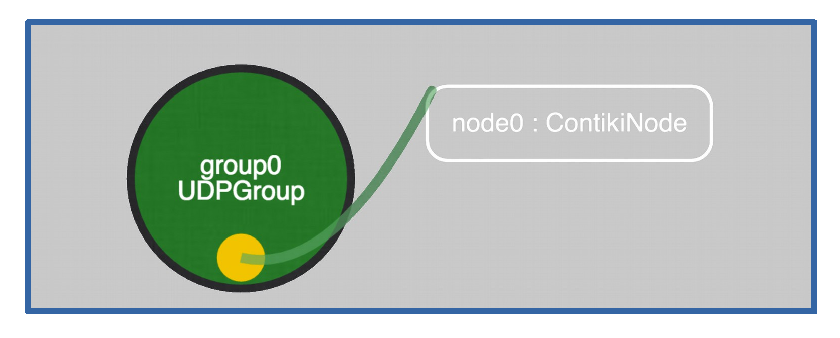
\includegraphics[width=0.55\columnwidth]{chapters/modelsAtRuntimeContiki.images/MAR_example.pdf}
	\caption{Graphical representation of a minimal M@R}
	\label{fig:1stModelC}
\end{figure}

Indeed, our efforts were put into a first manual implementation of the Kevoree meta-model.
The size of the test application which contains a group and a node without components is shown in table \ref{tab:kevoreeC}
A graphical representation of the model can be obtained through the Kevoree Web Editor\footnote{\url{http://editor.kevoree.org/v4/}}, in which a serialized JSON file containing the model can be loaded for edition.
This representation is shown in figure \ref{fig:1stModelC}.

%Our firsts results show that approximately 180KB of ROM space (text) are needed for the implementation, while 14KB of RAM (data + bss) were enough for such application.
%This test was compiled using the GCC (GNU C Compiler) version 4.9, for a i386 32-bit platform.
%Therefore, we need to find an IoT device which fit this minimal requirements.

It is then necessary to characterize the minimum system requirements for an IoT device to implement a full model@runtime middleware, as in hardware capabilities as in execution environment.
This will avoid the use of third party nodes to perform the high level tasks described above.
However, even if a proposed device meet the characteristics to perform such tasks, the trade-offs between energy consumption and the middleware execution should be taken into account.
A general description of needed features to execute the proposed middleware is given in the next subsection.

%\subsection{Needed features of the underlying system}
\subsection{Handling hardware constraints}
%Currently the concept of model@runtime has been applied on top of object oriented languages which offers the required features at the language level to implement the model@runtime layer. 
%The first challenge lies in the fact that Contiki does not support these object oriented languages and thus the design must fit a procedural language such as C.

%The second challenge lies in the very limited resources of the IoT nodes, thus forcing the middleware to meet the memory and CPU constraints. 
%This imposes constraints on the way the model is represented, stored and processed on each node.
%This challenge is particularly important and hard to meet, since many software components are needed to enable the communication in these environments (radio/MAC/IP stack and so on).
Given the challenges already stated in Section \ref{sec:kevAndIoT}, we must test our implementation on real hardware platforms in order to measure the limitation of our approach, as well as its compatibility with the other implementations (Java, Cloud, Android).
Moreover, the energy constraint of each IoT node, together with the mesh topology of the network makes communication in this environments fairly reliable.
This implies the necessity to optimize the way the model and the software are disseminated on the network.

At first glance, our implementation was compiled for three different platforms (\textit{class 1}): the \textit{\textbf{zolertia Z1\footnote{\url{http://zolertia.sourceforge.net/wiki/images/e/e8/Z1_RevC_Datasheet.pdf}}, redbee econotag\footnote{\url{http://redwire.myshopify.com/products/econotag-ii}} and wismote\footnote{\url{http://wismote.org/doku.php}}}}, which were widely used for research purposes in the IoT domain.
Unfortunately, none of these platforms was able to meet the space requirements in ROM and RAM to run a minimal model at runtime as shown in figure \ref{fig:1stModelC}.
However, the existence of more powerful microcontrollers, an essential part of an IoT device, shows that typical IoT applications have not exceeded the resources of existing experimentation platforms.
Indeed, only some development kits such as TI's CC2538DK\footnote{\url{http://www.ti.com/tool/cc2538dk}} were available at that time, but its high cost, low availability and poor support gave low acceptance for research purposes.
Thus, the design and construction of a new experimentation platform seemed to be the fastest way to obtain the first results of the implementation, by integrating the latest microcontrollers and peripherals available on the market.
It is worth to consider that this platform was conceived for research and experimentation purposes, and not as an end-user device.

An exhaustive search was conducted to find the latest technologies to build an experimentation IoT device, which fits the requirements already estimated in section \ref{subsec:MARImpl}.
The first step was to find the basic components of such a device.
Taking into account the requirements from section \ref{sec:MARMech4IoT}, an IoT device should, more specifically, embed:
\begin{enumerate}
	\item \textbf{Microcontroller.} A low-power microcontroller unit is needed to perform the computational processing tasks as well as to store the program code. 
	A huge amount of ROM and RAM is needed at the scale of these devices, thus it is necessary to find a microcontroller with a good trade-off between energy consumption and memory size.
	\item \textbf{Communication interface.} Communication is the main task that will perform our device, since it is mandatory for IoT environments.
	A radio interface implementing the widely used IEEE 802.1.5.4 standard\cite{ieee802.15.4} is then necessary to communicate in an interoperable way with other devices.
	An ultra-low energy consumption is also important, since communication is the most energy consuming task.
	\item \textbf{External flash memory.} Storage for data is a very useful feature for an IoT device. It can serve as persistent data storage for logging and data collection from sensors, as well as updates and eventually new firmwares.
	\item \textbf{Sensors and actuators.} In order to collect experimentation data, some sensors should be embedded on the device, the most common being temperature, humidity and position.
	Indicator LEDs are also commonly present in these devices, to provide visual signs such as function status (ON/OFF) or current communication.
	\item \textbf{Ports for external devices.} An easy way to connect third party devices allows a dynamic behavior, since we can connect other sensors, actuators and devices which cannot be present internally on the device.
	Such devices should be connected using standard interfaces, such as I2C and SPI.
	General Purpose Inputs/Outputs (GPIO) are also widely used, either as digital or analog interfaces.
	\item \textbf{Battery capabilities.} An IoT device is very often used in environments where a constant power source is not present.
	Thus, work on batteries is a very useful feature to test energy consumption while adding flexibility of placement.
\end{enumerate}

Given these features, it was then necessary to integrate several components in order to build the required IoT device.
We put special attention to the most critical components, which are the microcontroller, the external flash memory and the battery controller.
Regarding the radio transceiver and the other peripherals, there are no huge differences between the most commonly used, for instance, the ones used in the previously analyzed devices.
The specific conception of the platform will be described in the next subsection.

\subsection{Towards a new IoT device}
\label{subsec:newIoTDevice}
Several low-power microcontroller architectures were available at the time of our first M@R implementation, such as TI MSP430, Atmel AVR, Microchip PIC and ARM Cortex-M, just to mention the most common ones.
Since our middleware minimum memory requirements were tested on 16-bit MSP430 microcontrollers (Zolertia's Z1 and Arago's WiseMote), finding a huge scarcity of memory, 32-bit architectures were the target of our scope.
Indeed, ARM Cortex-M microcontrollers offer only 32-bit RISC architectures, which are widely used both in research and industry.
Thus, the first step was to select an ARM Cortex-M microcontroller fitting our memory and energy consumption requirements.
The ST Microelectronics STM32 family of microcontrollers offers a wide range of devices with different processor speeds and memory sizes.
%\begin{figure}[]
%	\centering
%	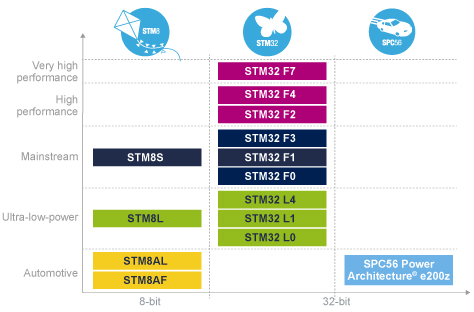
\includegraphics[width=0.70\columnwidth]{chapters/modelsAtRuntimeContiki.images/STM32.jpg}
%	\caption{STM32 Microcontroller family}
%	\label{fig:STM32}
%\end{figure}
%Figure \ref{fig:STM32} shows the STM32 family applications and available solutions for each one.

%At the time of this search, ultra-low-power solutions (STM32L) were not available, thus our possibilities were in the STM32F range, excluding the F7 which was also released recently.

\begin{table}[]
	\centering
	\caption{Comparison between STM32F microcontrollers}
	\label{tab:STM32F}
	\begin{tabular}{c|cccc}
		Microcontroller & Speed (MHz) & RAM (KB) & ROM (KB) & \begin{tabular}[c]{@{}c@{}}Consumption \\ at max. speed (mA)\end{tabular} \\ \hline
		STM32F0         & 48          & 32       & 256      & 22                                                                        \\
		STM32F1         & 72          & 96       & 1024     & 68                                                                        \\
		STM32F3         & 72          & 80       & 512      & 61.5                                                                      \\
		STM32F2         & 120         & 128      & 1024     & 49                                                                        \\
		STM32F4         & 180         & 256      & 2048     & 98                                                                       
	\end{tabular}
\end{table}

Since our goal is to build a device on which our experimentations could be executed on a more flexible way (without caring about memory requirements), it is preferable to use a microcontroller featuring the highest memory capabilities, both in ROM and RAM, over energy consumption.
Moreover, these kind of devices are able to change the processor speed as needed, thus reducing the energy consumption.
Indeed, our choice was a STM32F4 microcontroller, which was used as the core of our IoT device.
Table \ref{tab:STM32F} shows a comparison between the available microcontrollers, featuring the maximum processor speed, RAM and ROM, followed by the current consumption in such configuration.

As for the power scheme, given the capabilities of the selected microcontroller, a power source between 1.8V and 3.6V is required.
Indeed, a first approach to power the device is the use of an USB port, which delivers around 5V.
Thus, a 5V to 3.3V (the recommended tension) is required.
In contrast, when the device is needed to run on batteries, the supplied voltage will change.
%The most common batteries available on the market provide between 1.5V (AA, AAA) and 3V (CR3032), which is in the acceptable range.
A couple of AA batteries connected in series is the most standard array to power IoT devices, delivering 3V, enough for our device.
However, a wide set of peripherals such as sensors and actuators work very often at 5V.
Therefore, it was necessary to add a DC to DC converter, coupled with an automatic power selector which detects when the device is powered either by USB or batteries.
This allows to use any power scheme without decreasing performance or peripherals compatibility.

\begin{table}[]
	\scriptsize
	\centering
	\caption{IoT Platforms comparison}
	\label{tab:IoTPlatfComp}
	\begin{tabular}{cccccccc}
		\textbf{}                                                                               & \textbf{\begin{tabular}[c]{@{}c@{}}Speed \\ (MHz)\end{tabular}} & \textbf{\begin{tabular}[c]{@{}c@{}}RAM \\ (KB)\end{tabular}} & \textbf{\begin{tabular}[c]{@{}c@{}}ROM \\ (KB)\end{tabular}}                               & \textbf{\begin{tabular}[c]{@{}c@{}}External \\ flash (MB)\end{tabular}} & \textbf{\begin{tabular}[c]{@{}c@{}}Radio \\ transceiver\end{tabular}} & \textbf{Peripherals}                                                                                    & \textbf{\begin{tabular}[c]{@{}c@{}}Embedded\\ Sensors\end{tabular}}                                \\ \cline{2-8} 
		\multicolumn{1}{c|}{\textbf{\begin{tabular}[c]{@{}c@{}}Zolertia \\ Z1\end{tabular}}}    & \multicolumn{1}{c|}{16}                                         & \multicolumn{1}{c|}{8}                                       & \multicolumn{1}{c|}{96}                                                                    & \multicolumn{1}{c|}{2}                                                  & \multicolumn{1}{c|}{CC2420}                                           & \multicolumn{1}{c|}{\begin{tabular}[c]{@{}c@{}}UART, I2C\\ Phidgets \\ (USB only),\\ GPIO\end{tabular}} & \multicolumn{1}{c|}{\begin{tabular}[c]{@{}c@{}}3 axis acc.\\ and\\ temperature\end{tabular}}       \\ \cline{2-8} 
		\multicolumn{1}{c|}{\textbf{\begin{tabular}[c]{@{}c@{}}Arago's\\ WisMote\end{tabular}}} & \multicolumn{1}{c|}{25}                                         & \multicolumn{1}{c|}{16}                                      & \multicolumn{1}{c|}{256}                                                                   & \multicolumn{1}{c|}{8}                                                  & \multicolumn{1}{c|}{CC2520}                                           & \multicolumn{1}{c|}{\begin{tabular}[c]{@{}c@{}}UART, I2C,\\ Phidgets, \\ GPIO\end{tabular}}             & \multicolumn{1}{c|}{\begin{tabular}[c]{@{}c@{}}3 axis acc.\\ light and\\ temperature\end{tabular}} \\ \cline{2-8} 
		\multicolumn{1}{c|}{\textbf{\begin{tabular}[c]{@{}c@{}}Redbee\\ econotag\end{tabular}}} & \multicolumn{1}{c|}{26}                                         & \multicolumn{1}{c|}{96}                                      & \multicolumn{1}{c|}{\begin{tabular}[c]{@{}c@{}}N/A\\ (device run\\ from RAM)\end{tabular}} & \multicolumn{1}{c|}{128 (KB)}                                           & \multicolumn{1}{c|}{Integrated (SoC)}                                 & \multicolumn{1}{c|}{GPIO}                                                                               & \multicolumn{1}{c|}{N/A}                                                                           \\ \cline{2-8} 
		\multicolumn{1}{c|}{\textbf{\begin{tabular}[c]{@{}c@{}}DiverSE\\ Board\end{tabular}}}   & \multicolumn{1}{c|}{180}                                        & \multicolumn{1}{c|}{256}                                     & \multicolumn{1}{c|}{2048}                                                                  & \multicolumn{1}{c|}{16}                                                 & \multicolumn{1}{c|}{CC2520}                                           & \multicolumn{1}{c|}{\begin{tabular}[c]{@{}c@{}}UART (x2), \\ I2C\\ Phidgets, \\ GPIO\end{tabular}}      & \multicolumn{1}{c|}{N/A}                                                                           \\ \cline{2-8} 
	\end{tabular}
\end{table}

Thus far, the main required features for our device are met.
A comparison between the previously tested platforms and ours is given in table \ref{tab:IoTPlatfComp}, showing the most common useful features.
\todo{Add a photo of the device}
%Details about the other components such as the radio transceiver and the external flash memory can be found in \todo{annex X.}

Given the features of our new IoT device, the next step is to provide the hardware abstraction layer and a network stack to integrate it into an IoT network.
Indeed, several IoT operating systems existed at the time this device was developed, thus leveraging one of these available OS was the most recommended procedure.
%The next Subsection discuss the implementation of all the necessary tools to integrate our middleware into this new platform, making the choice of porting the Contiki OS to support our IoT device.
It is important to notice that our middleware implementation it's independent of the underlying OS, since it only provides abstractions for the representation of the running system in the form of a model@runtime.
Thus, it can be adapted to any other OS able to integrate modules written on C, as well as networking facilities typical of the IoT to disseminate such model.

\section{Kevoree software implementation requirements}
\label{sec:kevoreeRequirements}
Our middleware approach will need several features from the underlying system, in order to match with the high-level description provided by the model@runtime.
As we discussed on our state of the art in Section \ref{sec:IoTDeployment}, the most common approach used to run applications on IoT devices is bare-metal development followed by firmware flashing into the ROM memory.
Even if this method allows a fine control of the underlying hardware, the development time can be very long and difficult to debug, since abstractions are mostly done only at the hardware level, and does not come to the system level.
Moreover, since complexity grows, applications for IoT should be developed without special attention to hardware and system concerns.
Thus, an IoT operating system should be used, in order to leverage its system-level abstractions.

As presented in the state of the art, several IoT operating systems exist, but according to the needed features some of them are more convenient.
We can thus refine the requirements given in section \ref{sec:MARMech4IoT}, according to OS properties:
\begin{enumerate}
	\item \textbf{Basic OS functionalities such as timers, task scheduler and Inter Process Communication (IPC).} Basic functionalities that are the core of any embedded OS.
	\item \textbf{Dynamic linker and loader, following the third approach presented in section \ref{sec:IoTDeployment}.} A dynamic linker and loader is essential to our approach, since changes in the model containing new software components will trigger the download and instantiation of an artifact, which should be linked and loaded at runtime by the underlying system.
	\item \textbf{Network stack implementing basic IP functions (TCP, UDP, HTTP, CoAP).} In order to share a model and download software artifacts, IP communication is mandatory, since the goal is to use the Internet to reach component repositories from different sources.
	\item \textbf{Persistent data handling, preferably a file system.} The method used to avoid RAM storage is to serialize the model@runtime in a file on the flash memory, usually in the JSON format. Thus, a way to store and access this JSON file for reading and writing should be provided.
	\item \textbf{Abstractions for attached devices (LEDs, sensors, actuators, etc.).} Although not mandatory, an OS usually carry basic hardware abstractions, providing an easy way to develop applications which need a physical interaction with the external world.
\end{enumerate}
In order to make a rapid functional prototype of our middleware, we will make use of the Contiki OS which, given the features presented above, seems to fit our minimal requirements.
Despite the programming model already described as a drawback, Contiki offers all the needed functionalities, as well as a wide community which collaborate very actively in the development and debug of it.
%Therefore, we use the ContikiOS\cite{dunkels2004contiki} in order to provide an efficient way to distribute components, since it allows dynamic loading of binary modules.
Moreover, Contiki includes an implementation of 6loWPAN\cite{rfc4944}, an adaptation layer for an IPv6 compressed stack, which let us assign directly an IPv6 address to the device.
This enables a ready to use IoT environment.
Afterwards, an UDP transport layer is provided, allowing a standard way to reach UDP servers to download the needed deploy units to perform system adaptations, according to the model@runtime engine.
%We use erbium's\cite{rfc7252} CoAP implementation in order to have a REST engine which is used as a main communication channel between nodes. 
Indeed, one of the most important features provided by this OS is the dynamic code loading mechanisms.
These are based on a dynamic linker and loader that use the standard ELF object file format\cite{dunkels06runtime}.

However, even if the OS fulfill all the requirements, the computational resources needed by our middleware should be taken into account, in order to use a flexible hardware platform on which we can evaluate our approach.
As presented previously on this chapter, the minimum requirements for our first implementation have already been defined, resulting in the design of a new board.

\section{Summary}
At this point, we can highlight the main requirements and functionalities needed from a typical IoT device, as well in terms of software as in hardware, in order to run a models@runtime implementation.
We can now observe that the challenges are concentrated on the internal behavior of an IoT node, thus focusing only in providing an \textit{intra-node} implementation.
This intra-node view will guide us to put our efforts into a first proposal of the Kevoree-IoT middleware, taking into account all the design requirements exposed throughout this chapter.

It is important to notice and remember that our environment is very constrained, first in the intra-node perspective but also in the inter-node mechanisms.
Indeed, we can classify our challenges as following:

\begin{enumerate}
	\item \textbf{Intra-node challenges:} Memory, processing, storing and programming environment constraints.
	\item \textbf{Inter-node challenges:} Networking, thus communication, which impacts primary the energy consumption.
\end{enumerate}

Figure X provides a general view of these challenges, highlighting its place on the overall research work, stating our main goals.

The next chapter will provide the implementation details of our intra-node design specifications, followed by an evaluation of the possibilities and limitations of our approach.
Since our goal is to provide a middleware that works on real platforms, our evaluations were conducted, first, on our designed hardware platform.
Moreover, once our first tests are analyzed, we followed our research goals by testing our implementation on a large-scale testbed.
Indeed, this last evaluation will trigger the actual challenges for the inter-node needed mechanisms, which will be presented in the chapter afterwards.

%As a final consideration, the executed application contained a very minimalistic model, including only enough characteristics to manipulate such model.
%Indeed, for the next chapter, a more complete implementation of the modeling framework is proposed, resulting in a more robust middleware.
%For this reason, the size of the application can increase, and the ability to instantiate components and nodes at the model level can be decreased.
%The next chapter will explore the needed features at the system level to actually behave as self-adaptive, by enacting the adaptation plan provided by the M@R engine.
%Moreover, some crucial features available at the system level can be undetermined or incomplete, thus efforts to complete and provide all the necessary facilities should be done. 